\chapter{Elaboration}
\label{sec:related}

\hspace{0pt}
\vfill

\section{Use Case}
\subsection{Use Case Diagram}

\begin{figure}[h]
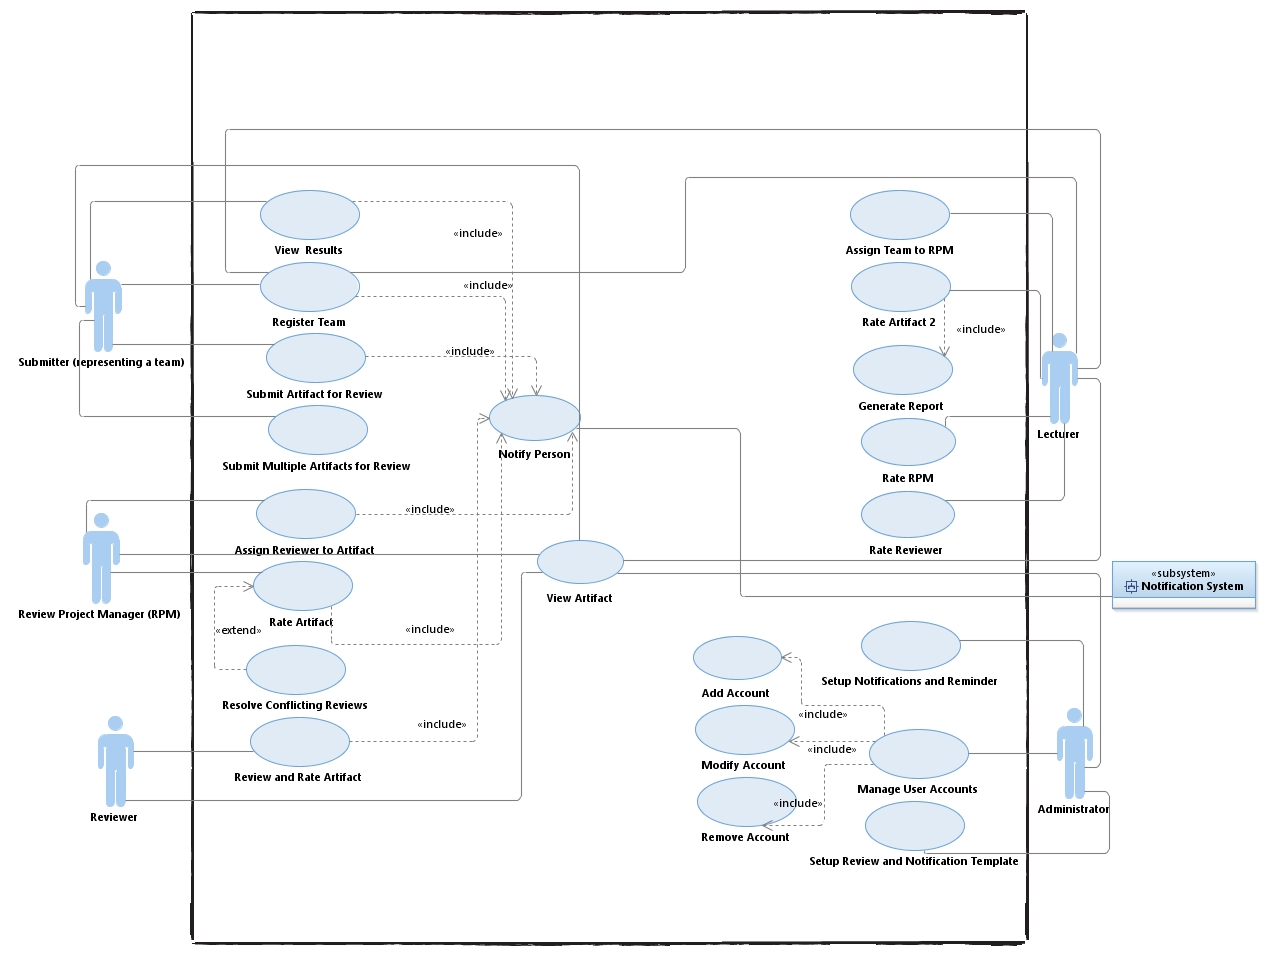
\includegraphics[width=17cm]{UseCase.jpeg}
\centering
\caption{Use Case Diagram of SoftProj System}
\end{figure}


\vfill
\hspace{0pt}
\pagebreak

\subsection{Fully Dressed Use Cases}
    \subsection*{Use Case UC1: Review Artifact (Reviewer)}
    \subsubsection*{Scope:} SoftProj Project Submission and Review System
    \subsubsection*{\textbf{Level:} }User Goal
    \subsubsection*{\textbf{Primary Actor:} } Reviewer
    \subsubsection*{\textbf{Stakeholders and Interests:}}
    \begin{itemize}
    \itemsep-1em 
        \item Reviewer: Wants to review an artifact by leaving a rating and description.
        \item RPM: Wants the reviewers assigned to the artifacts to leave a review.
         \item Lecturer: Wants RPM and reviewers to review assigned artifacts for a team.
          \item Submitter: Wants to receive reviews on their artifacts from the Reviewers, RPM, and Lecturer
         \item System: Wants to notify Reviewers when they have been assigned to submit a
       review for a new Artifact.
    \end{itemize}
    
    
    \subsubsection*{\textbf{Preconditions:}}
    \begin{itemize}
    \itemsep-1em 
        \item Reviewer is identified and authenticated.
        \item Reviewer has been assigned by an RPM to review an Artifact submitted by a
        Team.
         \item Reviewer is notified by the System that they have been assigned to review an
          Artifact.
        \item Reviewer has access to the Review Template for the Artifact Type for which they are going to review.
        \item Reviewer has access to the Artifact for which they are going to review.
    \end{itemize}


    
    
    
    \subsubsection*{Success Guarantee (Postconditions):}
    \begin{itemize}
    \itemsep-1em 
       \item A Review was created by the Reviewer for the associated Artifact.
       \item The Review created includes a rating and a description of the review.
\item The RPM, Lecturer, and Team were notified about the newly created review for
        the Artifact with which they are associated.
    \end{itemize}
    
    
    
    \subsubsection*{Main Success Scenario (Basic Flow):}
    \begin{enumerate}
        \itemsep-1em 
        \item Reviewer is notified by the System that they need to review a specific Artifact. \textbf{Includes Notify Person}
        \item Reviewer logs into the System and views the Artifact they have been assigned
         to review. \textbf{Includes View Artifact}
        \item Reviewer writes and submits a rating and description for the given Artifact.
         \item Reviewer publishes their review.
         \item The Reviewer gets confirmation from the System that their Review was
          published.
          \item The System notifies other Users associated with the Artifact who are subscribed to notifications about that artifact. \textbf{Includes Notify Person}
    \end{enumerate}
    
    
    
    
     \subsubsection*{Extensions (Alternative Flows)}\textbf{:}
     \newline
     \\
     3a. Unpulished Review Submission
     \begin{enumerate}
         \itemsep-1em 
        \item Reviewer may submit an unfinished Review to the System.
         \item Reviewer completes the Review at a later time.
         \item When Reviewer has completed Review, they publish the Review.
          \item Execution in Main Success Scenario step 5 continues.
    \end{enumerate}
    5a. System is unable to Publish Review because a part was not completed or data was
not received by the server:
\begin{enumerate}
        \itemsep-1em 
        \item System tells Reviewer what the error was with their attempted published
        submission.
        \item Since Review was not published, execution goes back to Main Success Scenario
         step 3.
    \end{enumerate}


\subsubsection*{Special Requirements:}
    \begin{itemize}
    \itemsep-1em 
       \item Reviewer has access to a computer which can access the System and will allow
         them to view the Artifact and write the Review.
       \item The change history of a Review is kept so that a Reviewer may revert to an earlier Review submission before publishing.
    \end{itemize}
     

     \subsubsection*{Technology and Data Variations List}\textbf{:}
     \\
     \\
     1. \& 5. Notifications may be received on multiple devices connected to the System via
     the internet.
      \\
     3. Reviewer writes Review in the language specified for the course.
     
     \subsubsection*{Frequency of Occurrence}\textbf{:}
     \\
     \\
     Multiple times a day or not at all in a single day. As quickly as Reviewers can write Reviews for Artifacts which they are assigned.
     
     
     
     \subsubsection*{Open Issues:}
    \begin{itemize}
    \itemsep-1em 
       \item What if a Reviewer wants to change their Review? Can they “Re-Publish”?
       \item What if a Reviewer never submits their Review?
       \item What if a Reviewer is never assigned to Review an artifact?
    \end{itemize}
    
    
    
    %newusecase2
    
    
    
    \subsection*{Use Case UC2: Assign Team to RPM}
    \subsubsection*{Scope:} SoftProj Project Submission and Review System
    \subsubsection*{\textbf{Level:} }User Goal
    \subsubsection*{\textbf{Primary Actor:} } Lecturer
    \subsubsection*{\textbf{Stakeholders and Interests:}}
    \begin{itemize}
    \itemsep-1em 
        \item Lecturer: Wants to assign an RPM to manage the reviewing of all artifacts for a given Team.
        \item RPM: Wants to get assigned to manage the reviewing all artifacts for 1 or more Teams. Wants to tell Reviewers to write Reviews for the assigned Team’s Artifacts.
         \item Team \& Submitters: Wants their Artifacts to get reviewed.
          \item Wants to notify RPMs and teams when they are associated with one another.
        
    \end{itemize}
    
    
    \subsubsection*{\textbf{Preconditions:}}
    \begin{itemize}
    \itemsep-1em 
        \item Lecturer is identified and authenticated. 
        \item Lecturer manages a group of RPMs who have been identified and authenticated from which they can choose to assign to Teams.
         \item Lecturer manages a group of Teams who have been identified and authenticated to which they can assign RPMs.
        \item Lecturer is notified the first time a Team submits an Artifact so that the Lecturer may assign an RPM to the team.
        \item The Team who is going to have the RPM assigned to them must have submitted an Artifact which needs review.
    \end{itemize}


    
    
    
    \subsubsection*{Success Guarantee (Postconditions):}
    \begin{itemize}
    \itemsep-1em 
       \item An RPM has been assigned to the Team which submitted their first artifact..
       \item The Team has been notified that an RPM has been assigned to them if they subscribe to these notifications.
\item The RPM has been notified that they have been assigned to a team and that they need to begin assigning Reviewers to the Team’s Artifacts.
    \end{itemize}
    
    
    
    \subsubsection*{Main Success Scenario (Basic Flow):}
    \begin{enumerate}
        \itemsep-1em 
        \item Lecturer is notified by the System that a Team has submitted their first Artifiact and that the Lecturer needs to assign an RPM to that Team. \textbf{Includes Notify Person}
        \item Lecturer logs into the System and sees which Team needs to be assigned an RPM and which RPMs are available to be assigned.
        \item Lecturer chooses an RPM to assign to the Team and submits this decision to the System.
         \item System gives the Lecturer confirmation that their decision has been recorded.
         \item The Team and RPM all receive notifications of being assigned to one another if they are subscribed to notifications about this. \textbf{Includes Notify Person}
    \end{enumerate}
    
    
    
    
     \subsubsection*{Extensions (Alternative Flows)}\textbf{:}
     \newline
     \\
     2a. Team no longer exists
     \begin{enumerate}
         \itemsep-1em 
        \item If the Team has been deleted or removed from the System before they could be Assigned an RPM, the Lecturer will no longer see this Team as needing to be assigned an RPM.
    \end{enumerate}
    2b. Team revoked their Artifact submission
\begin{enumerate}
        \itemsep-1em 
        \item If the Team revoked their Artifact submission, the Lecturer may still proceed in assigning an RPM to the team.
    \end{enumerate}
    
    2c. No RPMs available
    
    \begin{enumerate}
        \itemsep-1em 
        \item If no RPMs exist in the System or are available, it will be impossible for the Lecturer to assign an RPM to the team, so this flow must end until RPMs become available.
    \end{enumerate}
4a. System fails to confirm Lecturer’s decision and says the decision was not recorded:
    
    \begin{enumerate}
        \itemsep-1em 
        \item System tells Lecturer what the error or if the decision did not submit to the server.
        \item Since RPM and Team pairing decision was not published, execution goes back to Main Success Scenario step 3.
    \end{enumerate}
    


\subsubsection*{Special Requirements:}
    \begin{itemize}
    \itemsep-1em 
       \item Lecturer has access to a computer which can access the System and will allow them to see existing RPMs and Teams which they may assign together.
    \end{itemize}
     

     \subsubsection*{Technology and Data Variations List}\textbf{:}
     \\
     \\
     1. \& 5. Notifications may be received on multiple devices connected to the System via
     the internet.
      \\
     
     
     \subsubsection*{Frequency of Occurrence}\textbf{:}
     \\
     \\
     Multiple times a day or not at all in a single day. As quickly as Team’s submit their first Artifact for Review and RPMs are available to be assigned to Teams.
     
     
     
     \subsubsection*{Open Issues:}
    \begin{itemize}
    \itemsep-1em 
       \item Can the Lecturer Re-assign a team to a different RPM?
       \item Can an RPM be assigned to multiple Teams?
       \item What can the Lecturer do when no RPMs are available to be assigned?
       \item Could the Lecturer simply assign an RPM after a Team has been created instead of after the first Artifact is submitted? This could cause some latency in the Review process.
    \end{itemize}









\newpage

%USECASE3


    
    
    
    
    
    
     \subsection*{Use Case UC3: Register Team}
    \subsubsection*{Scope:} SoftProj Project Submission and Review System
    \subsubsection*{\textbf{Level:} }User Goal
    \subsubsection*{\textbf{Primary Actor:} } Submitter
    \subsubsection*{\textbf{Stakeholders and Interests:}}
    \begin{itemize}
    \itemsep-1em 
        \item Submitter: Wants to make registration as a team for future submission.
        \item Lecturer: Wants to approve registration of the team for their submission.
         \item System: Wants to notify the team after registration.
    \end{itemize}
    
    
    \subsubsection*{\textbf{Preconditions:}}
    \begin{itemize}
    \itemsep-1em 
        \item Submitter is eligible to make registration as a team.
        \item Submitter is also the member of the team.
         \item Lecturer is identified and authenticated.
        \item Lecturer is not the submitter.
    \end{itemize}
    
    


    
    
    
    \subsubsection*{Success Guarantee (Postconditions):}
    \begin{itemize}
    \itemsep-1em 
       \item Team is registered.
       \item The team list is updated.
       \item Project can be submitted by team
       
    \end{itemize}
    
    
    
    \subsubsection*{Main Success Scenario (Basic Flow):}
    \begin{enumerate}
        \itemsep-1em 
        \item Submitter applies for registration as a team.
        \item When applying submitter gives the information of the team members.
        \item The system sends email to all the team members for verification.
         \item All team members verify, and the system sends notification to Lecturer. 
         \item Lecturer approves their registration.
          \item System notifies all team members individually that their team has been registered. 
          \item The system updates the information.
    \end{enumerate}
    
    
    
    
     \subsubsection*{Extensions (Alternative Flows)}\textbf{:}
     \newline
     \\
     4a. Any team member does not verify:
     \begin{enumerate}
         \itemsep-1em 
        \item The system waits for two days and then again sends email to that member for verification.
        \\
        1a. Team member verifies, and system proceeds to the next step.
        \\
        1b.Team member does not respond after two days of the second email:
        \begin{enumerate}
            \item The system notifies the submitter and cancels their application.
        \end{enumerate}
    \end{enumerate}
    


\subsubsection*{Special Requirements:}
    \begin{itemize}
    \itemsep-1em 
       \item Submitter has access to see team’s registration progress.
    \end{itemize}
     

     \subsubsection*{Technology and Data Variations List}\textbf{:}
     \\
     \textbf{1a.} Submitter applies using his/her own device via internet.
     \\
     \textbf{4a.} Team members verifies their email using multiple or single device via internet.
     \\
    \textbf{ 5a.} Lecturer uses his/her own device
     \\
     \textbf{6a.} Notifications may be received on multiple devices connected to the System via internet.
     
     \subsubsection*{Frequency of Occurrence}\textbf{:}
     \\
     \\
     Multiple  times  a  day  or  not  at  all  in  a  single  day.  As  quickly  as Team  completes  application Lecturer approves it.
     
     
     
     \subsubsection*{Open Issues:}
    \begin{itemize}
    \itemsep-1em 
       \item Can a submitter team consist of only one student? 
       \item If any team member misses to verify the his/her email address after $2^{nd}$ email, will the team be able to apply again?
       \item What happens when Lecturer is not available to approve the team registration?
    \end{itemize}
    
    
    
    
    
    
    
    
    %usecase4
    
    
    \newpage 
    
     \subsection*{Use Case UC4: Submit Artifact for Review}
    \subsubsection*{Scope:} SoftProj Project Submission and Review System
    \subsubsection*{\textbf{Level:} }User Goal
    \subsubsection*{\textbf{Primary Actor:} } Submitter
    \subsubsection*{\textbf{Stakeholders and Interests:}}
    \begin{itemize}
    \itemsep-1em 
        \item Submitter: Wants to make submission for being reviewed.
        \item Lecturer: Wants to assign this submission to a specific RPM.
         \item System: Wants to notify the Lecture after submission and the RPM after assigning him/her to a new submission.
    \end{itemize}
    
    
    \subsubsection*{\textbf{Preconditions:}}
    \begin{itemize}
    \itemsep-1em 
        \item Lecturer is identified and authenticated.
        \item Submitter is identified and authenticated.
         \item RPM is identified and authenticated.
        \item Lecturer is not the submitter.
        \item RPM is not the submitter.
    \end{itemize}
    
    


    
    
    
    \subsubsection*{Success Guarantee (Postconditions):}
    \begin{itemize}
    \itemsep-1em 
       \item Artifacts are submitted.
       \item The team members have been notified after submission.
       
    \end{itemize}
    
    
    
    \subsubsection*{Main Success Scenario (Basic Flow):}
    \begin{enumerate}
        \itemsep-1em 
        \item Submitter submits the artifact and fill out a template with information about the artifact.
        \item The system verifies that the Lecturer and the Submitter are not the same person
        \item System notifies the Lecturer about this submission
         \item The lecturer finds an RPM for this submission 
         \item The system notifies the team members about the completion of their submission  
    \end{enumerate}
    
    
    
    
     \subsubsection*{Extensions (Alternative Flows)}\textbf{:}
     \newline
     \\
     \textbf{1a. }The system does not recognize the submitter as registered team:
     \begin{enumerate}
         \itemsep-1em 
        \item The system asks the submitter to register.
        \item The submitter makes registration and then submits.
    \end{enumerate}
    
    
  \textbf{1b.}Submitter does not fill out the template
     \begin{enumerate}
         \itemsep-1em 
        \item System notifies person to fill out the template.
    \end{enumerate}
    
    
   \textbf{ 2a.} Lecturer and submitter are the same person
    
    \begin{enumerate}
         \itemsep-1em 
        \item 1.The system recognizes this submission as a file which is not for review.
    \end{enumerate}
    
    
    \textbf{4a.} Submitter is from the team of RPM
    
    \begin{enumerate}
         \itemsep-1em 
        \item Lecturer assigns RPM accept that person.
    \end{enumerate}
    
    


\subsubsection*{Special Requirements:}
    \begin{itemize}
    \itemsep-1em 
       \item Submitter has access to see their submission’s current status.
    \end{itemize}
     

     \subsubsection*{Technology and Data Variations List}\textbf{:}
     \\
    \textbf{ 1a}. Submitter submits using his/her own device via internet.
     \\
     \textbf{2a.} System verifies using its database.
     \\
     \textbf{3a.} Lecturer receives notification in his/her own device via internet.
     \\
     \textbf{6a.} Notifications may be received on multiple devices connected to the System via internet.
     
     \subsubsection*{Frequency of Occurrence}\textbf{:}
     \\
     \\
     Multiple times a day or not at all in a single day. As quickly as Team makes submission system confirms it.
     
     
     
     \subsubsection*{Open Issues:}
    \begin{itemize}
    \itemsep-1em 
       \item Can a submitter resubmit his/her artifacts? 
       \item Can submitter submit artifacts after the deadline?
       \item What happens when Lecturer is not available to see the submission?
    \end{itemize}
    
    
    
    %usecase5
    \newpage
    
    \subsection*{Use Case UC5: Assign Reviewers to Artifact(s)}
    \subsubsection*{Scope:} SoftProj Project Submission and Review System
    \subsubsection*{\textbf{Level:} }User Goal
    \subsubsection*{\textbf{Primary Actor:} } Review Project Manager (RPM)
    \subsubsection*{\textbf{Stakeholders and Interests:}}
    \begin{itemize}
    \itemsep-1em 
        \item RPM: Wants to assign the reviewers to the artifact, so that reviewers can review it.
        \item Submitter:  Wants the artifact to be reviewed and rated.
         \item Reviewer:  Wants to be assigned to the artifact, so that he/she can review it.
          \item Lecturer:  Wants RPM to assign the reviewers to the artifact after it’s submitted.
         \item System:  Wants to notify reviewers when they are assigned to the artifact.
    \end{itemize}
    
    
    \subsubsection*{\textbf{Preconditions:}}
    \begin{itemize}
    \itemsep-1em 
        \item RPM is identified and authenticated.
        \item Submitter had submitted Artifact(or multiple Artifacts) for Review.  
         \item Lecturer had assigned Team to RPM. 
        \item RPM was notified that the artifact was submitted.  RPM was identified and authenticated.
    \end{itemize}


    
    
    
    \subsubsection*{Success Guarantee (Postconditions):}
    \begin{itemize}
    \itemsep-1em 
       \item At least two reviewers were assigned to the artifact by RPM. 
       \item Deadline was set for each reviewer to review the artifact. 
        \item Each reviewer was notified that he/she was assigned to the artifact.
        
    \end{itemize}
    
    
    
    \subsubsection*{Main Success Scenario (Basic Flow):}
    \begin{enumerate}
        \itemsep-1em 
        
        \item RPM logs in into the system.
        \item RPM sees which artifact was submitted.
        \item  System provides the list of candidate reviewers.
        \item  RPM decides how many reviewers will review the artifact.
        \item  RPM assigns at least two reviewers to the artifact.
        \item  RPM sets deadline for each reviewer.
        \item  System removes assigned reviewers from candidate reviewers list.
        \item System notifies each assigned reviewers that they were assigned to the artifact.  \textbf{Include Notify Person}
        \item  System sends confirmation to the RPM.
        \item  RPM leaves the system.
        
    \end{enumerate}
    
    
    
    
     \subsubsection*{Extensions (Alternative Flows)}\textbf{:}
     \newline
     \\
     \textbf{2-5a.} Multiple Artifacts were submitted:
     \begin{enumerate}
         \itemsep-1em 
        \item RPM sees which artifacts was submitted.
         \item System provides the list of candidate reviewers.
         \item RPM assigns reviewer to each artifact.
         \begin{enumerate}
         \itemsep-1em 
        \item RPM asks the system to notify when the number of candidate reviewers is greater than or equal to the number of artifacts submitted.
         \item System notifies RPM when the number of candidate reviewers is greater than or equal to the number of artifacts submitted.
         \item Use Case UC5 re-starts.
         
    \end{enumerate}
    
    \item Continue with step 6.
         
    \end{enumerate}
    
    
   \textbf{5a.}There are less than two candidate reviewers in the list:
\begin{enumerate}
        \itemsep-1em 
        \item RPM asks the system to notify when there are at least two reviewers in the candidate reviewerslist.
        \item System notifies RPM when there are at least two reviewers in the candidate reviewers list.3.
        \item Use Case UC5 re-starts.
    \end{enumerate}


\subsubsection*{Special Requirements:}
    \begin{itemize}
    \itemsep-1em 
    
    \item RPM has access to a computer which can access the System.
    \item  System works on various software platforms.
    \item  System provides different language options.
    \item System has user-friendly User Interface.
        
    \end{itemize}
     
\newpage
     \subsubsection*{Technology and Data Variations List}\textbf{:}
     \\
     \\
     \textbf{1.} RPM uses the account(username, password) created to him/her by Administrator.
     \\
     \textbf{6.} Deadline is set as exact date and time.  The format of the date and time changes according to the country the system is used.
     \\
     \textbf{8.} Notifications may be received on multiple devices connected to the System via the internet.
     
     \subsubsection*{Frequency of Occurrence}\textbf{:}
     \\
     \\
     Assuming that each submitter have to submit the artifact(s) each week (like in Software Engineering course), it occurs multiple times in a week.
     
     
     
     \subsubsection*{Open Issues:}
    \begin{itemize}
    \itemsep-1em 
       \item What if there are always less candidate reviewers than the number of artifacts in multiple artifacts submission case.
       \item Can RPM change his decision and re-assign the reviewers?
       \item  Can reviewer ask RPM to re-assign him/her to another artifact.
       \item  How candidate reviewers list is handled?  What are the rules for reviewer to be candidate reviewer?
    \end{itemize}
    
    
    
    %USECASE6
    
    \subsection*{Use Case UC6: Rate Artifact (RPM)}
    \subsubsection*{Scope:} SoftProj Project Submission and Review System
    \subsubsection*{\textbf{Level:} }User Goal
    \subsubsection*{\textbf{Primary Actor:} } Review Project Manager (RPM)
    \subsubsection*{\textbf{Stakeholders and Interests:}}
    \begin{itemize}
    \itemsep-1em 
    
    
    \item RPM: Wants to rate the artifact.
    \item  Submitter:  Wants the artifact to be reviewed and rated.
    \item  Reviewer:  Wants the artifact to be rated after he/she submits the review for the artifact.
    \item  Lecturer:  Wants to be notified when RPM rates the artifact.
    \item  System:  Wants to notify lecturer when RPM rates the artifact.
         
    \end{itemize}
    \newpage
    
    \subsubsection*{\textbf{Preconditions:}}
    \begin{itemize}
    \itemsep-1em 
        \item RPM is identified and authenticated.
        \item Each reviewer assigned to the artifact reviewed and rated the artifact.  
         \item RPM was notifiedthat each reviewer assigned to the artifact submitted their reviews. 
    \end{itemize}


    
    
    
    \subsubsection*{Success Guarantee (Postconditions):}
    \begin{itemize}
    \itemsep-1em 
       \item RPM rated the artifact. 
       \item Lecturer was notified that RPM rated the artifact. 
       \item Each reviewer of the artifact was notified that their reviews were accepted and the artifact was rated by RPM.
    \end{itemize}
    
    
    
    \subsubsection*{Main Success Scenario (Basic Flow):}
    \begin{enumerate}
        \itemsep-1em 
        \item RPM logs in into the system.
        \item  System shows all reviews submitted by reviewers of the artifact.
        \item  RPM reads each review.
        \item  RPM accepts each review.
        \item  RPM rates the artifact.
        \item  System notifies each assigned reviewers that their reviews were accepted and the artifact was rated by RPM. \textbf{Includes Notify Person}
        \item  System notifies lecturer that the artifact was rated by RPM. \textbf{Includes Notify Person}
        \item  System sends confirmation to the RPM.
       \item  The RPM leaves the system.
    \end{enumerate}
    
    
    
    
     \subsubsection*{Extensions (Alternative Flows)}\textbf{:}
     \newline
     \\
     \textbf{4a.} One or more reviews are not finished or are not according to review template:
     \begin{enumerate}
         \itemsep-1em 
        \item RPM rejects the one or more reviews.
        \item RPM looks which review has a problem.
        \item RPM rejects the review that has a problem.
        \item System  notifies  the  reviewer,  whose  review  has  a  problem,  that  he/she  needs  to  re-submit  the review.
    \end{enumerate}

            
        
        \newpage


\subsubsection*{Special Requirements:}
    \begin{itemize}
    \itemsep-1em 
       \item Reviewers had submitted the reviews using review template.
       \item  RPM has access to a computer which can access the System.
       \item  System works on various software platforms.
       \item  System provides different language options.
       \item  System has user-friendly User Interface.
    \end{itemize}
     

     \subsubsection*{Technology and Data Variations List}\textbf{:}
     \\
     \\
     \textbf{1.} RPM uses the account(username, password) created to him/her by Administrator.
      \\
      \textbf{5,6.} Notifications may be received on multiple devices connected to the System via the internet.
     \subsubsection*{Frequency of Occurrence}\textbf{:}
     \\
     \\
     Multiple times a week.  Can occur multiple times a day.
     
     
     
     \subsubsection*{Open Issues:}
    \begin{itemize}
    \itemsep-1em 
       \item Can RPM change his decision and rate the artifact again before lecturer rates and reviews the artifact,reviewers and RPM?
       \item Can RPM change his decision and reject the review of one or more reviewers after he/she rated the artifact?  Can he/she cancel the result of his/her rating?
    \end{itemize}
    
    
    
    
    
    
    
    
    
    
    
    
    
    
    
    
    
    
    
    
    
    
    
    
    
    
    %USECASE7
    \subsection*{Use Case UC7: Rate Artifact 2 (Lecturer)}
    \subsubsection*{Scope:} SoftProj Project Submission and Review System
    \subsubsection*{\textbf{Level:} }User Goal
    \subsubsection*{\textbf{Primary Actor:} } Lecturer
    \subsubsection*{\textbf{Stakeholders and Interests:}}
    \begin{itemize}
    \itemsep-1em 
        \item Lecturer: Wants to view the reviews, rate the artifact, the RPM \& the reviewers.
        \item Submitter: Wants to receive reviews on the artifacts from the Reviewers, RPM,and Lecturer
         \item System: Wants to notify submitter when an artifact has been rated.
          \item RPM: Wants the lecturer to view the reviews and then rate the artifact
         
    \end{itemize}
    
    
    \subsubsection*{\textbf{Preconditions:}}
    \begin{itemize}
    \itemsep-1em 
        \item Lecturer is identified and authenticated.
        \item Lecturer is notified by the System that there is an artifact left to be rated or he is notified when an artifact has been rated by an RPM
         \item Lecturer has access to the Review Template for the Artifact Type which he is going to rate.
        \item Lecturer has access to the Review template for rating the RPM and the reviewers.
        \item Lecturer has access to the Artifact which he is going to rate.
    \end{itemize}


    
    
    
    \subsubsection*{Success Guarantee (Postconditions):}
    \begin{itemize}
    \itemsep-1em 
       \item A Rate for the artifact has been given by the lecturer.
       \item The RPM and the associated reviewers have been rated by the lecturer.
\item The Rating for the artifact has been stored in the system.
\item The submitter has been notified that the artifact has been rated.
    \end{itemize}
    
    
    
    \subsubsection*{Main Success Scenario (Basic Flow):}
    \begin{enumerate}
        \itemsep-1em 
        \item Lecturer is notified by the System that he needs to view the reviews of an artifact \& then rate it.  \textbf{Includes Notify Person}
        \item Lecturer logs into the System. 
        \item Lecturer views the reviews given by the Reviewers for that artifact.
         \item Lecturer views the review given by the RPM for that specific artifact.
         \item Lecturer rates the artifact, the RPM and the Reviewers and then submits.
          \item The system saves the ratings.
          \item The system notifies the submitter that the artifact has been rated. \textbf{Includes Notify Person}
          \item The System confirms the lecturer that the rating has been saved
    \end{enumerate}
    
    
    
    
     \subsubsection*{Extensions (Alternative Flows)}\textbf{:}
     \newline
     \\
     2a.The profile/session of the Lecturer does not exist: 
     \begin{enumerate}
         \itemsep-1em 
        \item System notifies the lecturer of the error.
         \item The lecturer reboots the system.
    \end{enumerate}
    \newpage
    \textbf{3a.} Lecturer did not get reviews from one/all of the reviewers.
\begin{enumerate}
        \itemsep-1em 
        \item The Lecturer notifies the RPM of this error.\\
        \\
       \textbf{ 2a.} The RPM checks the saved reviews and finds the reviews
        \begin{enumerate}
            \itemsep-1em 
            \item The RPM notifies the Lecturer.
            \item The Lecturer notifies the Admin of this fault.
            \item The Admin then reviews the Access Control features.
        \end{enumerate}
       \textbf{ 2b.} The RPM failed to find the reviews:
        \begin{enumerate}
              \itemsep-1em 
            \item The RPM requests the reviewers to re-submit reviews
        \end{enumerate}
    \end{enumerate}
    
    \textbf{4a.} The RPM did not rate the Artifact:
    
     \begin{enumerate}
              \itemsep-1em 
            \item The Lecturer notifies the RPM of this error.
            \\
            \\
           \textbf{ 2a.} The RPM checks his records and finds the Rate
            \begin{enumerate}
            \itemsep-1em 
                \item The RPM notifies the Lecturer.
                \item The Lecturer notifies the Admin of this fault.
                \item The Admin then reviews the Access Control features.
            \end{enumerate}
           
           \textbf{ 2b.} The RPM failed to find the record of the Rate:
            \begin{enumerate}
            \itemsep-1em 
                \item The RPM views the Reviews and rates the Artifact.
                \item System sends notification to the Lecturer.
            \end{enumerate}
        \end{enumerate}
        
        \textbf{6a.} The system fails to save the rates given by the lecturer.
        \begin{enumerate}
            \itemsep-1em 
                \item The system notifies the lecturer.
                \item The system returns to a state prior to submission of the rate
                \item The process continues from step 5.
            \end{enumerate}
        
        \textbf{7a.} The system fails to notify:
        \begin{enumerate}
            \itemsep-1em 
                \item The system tries again.
                \item When done, the system lets the lecturer know that the submitter has been notified.
            \end{enumerate}
            
        
        


\subsubsection*{Special Requirements:}
    \begin{itemize}
    \itemsep-1em 
       \item Lecturer has access to a computer which can access the System and will allow him to view the Artifact and publish the rates.
         them to view the Artifact and write the Review.
       \item The change history of Rating is kept so that a Lecturer may revert to an earlier.
       \item Rating submission before publishing.
    \end{itemize}
     

     \subsubsection*{Technology and Data Variations List}\textbf{:}
     \\
     \\
     \textbf{1. \& 7.} Notifications may be received on multiple devices connected to the System via the internet.
      \\
     \subsubsection*{Frequency of Occurrence}\textbf{:}
     \\
     \\
     Multiple times a day or not at all in a single day. 
     
     
     
     \subsubsection*{Open Issues:}
    \begin{itemize}
    \itemsep-1em 
       \item What if a Lecture wants to change the rate? Can he“Re-Publish”rate?
       \item What if a Lecturer never submits his Rating?
       \item What if a Lecturer does not want to rate the Artifact, the RPM \& the reviewers at the same time?
    \end{itemize}
    
    
    
    
    
    
    
    
    
    
    
    %newsection
    
    
    \subsection{Casual Use Cases:}
    
    \subsection*{Use Case 8: Review RPM (Rate RPM)}
    The Lecturer wants to rate the performance of an RPM after the RPM has managed the Review process for a given Artifact and left a review. The Lecturer wants to make a “Person Review” for this RPM based on how well they managed the review process for an Artifact submitted by a Team. The Lecturer wants to give a rating and possibly a description in this Person Review which will be associated with the RPM.
    \\
    \\
    First an RPM manages the review process for an Artifact submitted by a team. When all Reviewers have submitted their Reviews, the RPM also submits their own review. The Lecturer is notified about the RPM’s submitted Review and reviews the Artifact herself/himself. Finally, the Lecturer can review the RPM’s performance by creating a “Person Review” which includes a rating and a description of their performance. This “Person Review” is then available for the RPM and Lecturer to see.
    
    
    \subsection*{Use Case 9: Review Reviewer (Rate Reviewer) }
    The Lecturer wants to rate the performance of a Reviewer after the Reviewer has written a Review for a given Artifact and the RPM has also left their review. The Lecturer wants to make a “Person Review” for this Reviewer based on how well they did their job. The Lecturer wants to give a rating and possibly a description in this Person Review which will be associated with the Reviewer.
    \\
    \\
    First a Reviewer is assigned to review an Artifact submitted by a team. Once the Reviewer has submitted their Review and the RPM has submitted their review, the Lecturer is notified about the RPM’s submitted Review and reviews the Artifact herself/himself. Finally, the Lecturer can review the Reviewer’s performance by creating a “Person Review” which includes a rating and a description of their performance. This “Person Review” is then available for the Reviewer and Lecturer to see.
    
    
    
    \subsection*{Use Case 10: Setup Review Template  }
    The Admin wants to setup Review Templates for various documents to be easily reviewable. The Admin wants to associate specific Artifact Types with Review Templates so that when someone comes to Review an artifact of a given Artifact Type, they have a Review Template to follow.
    \\
    \\
    First created Review Templates must exist for the admin to add to the System. Next, the Admin can upload a Review Template to the System and specify for which Artifact Types it may be associated with. Now any Lecturer, RPM, or Reviewer may see these Review Templates when they go to review an Artifact of the associated Artifact type.
    
    
    
    
    
    
    
    
    
    
    \subsection*{Use Case 11: Setup Notification Template  }
    The Admin wants to setup a Notification Template for any User to subscribe to a templatized set of Notifications. User’s want to be subscribed to receive Notifications to various information regarding their associations.
    \\
    \\
    First the Admin must be able to see all possible Notification Types, so that they may choose which Notifications should be present in a given Notification Template. The Admin may then create a new Notification Template. In this Template, they may select which Notifications should be enabled when a User is subscribed to this Template. The Admin can then submit the template which will become available for Users to see in their Notification settings. A User may then select a Notification Template to subscribe to so that they may receive certain types of Notifications which apply to them.
    
    
    
    
    
    
    
    
    
    
    
    
    
    \subsection*{Use Case 12: Generate Report (Lecturer) }
    The Lecturer is logged into the system. He wants to generate a report on current/past assignments to RPMs/Reviewers. The lecturer sends a request to the system with the Name/ID of the RPM/Reviewer to see the report. The system retrieves all the records for the specified person and the specified type of assignment and sends the list to the Lecturer. The Lecturer then views the report and if the lecturer wants then he can print the report or save it.
    \\
    \\
    The lecturer wants to generate report for the history of artifact submitted by a team. The lecturer sends this request to the system with the team-name/submitter-name. The system retrieves all the records for the specified person/team and sends the list to the Lecturer. The Lecturer then views the report and if the lecturer wants then he can print the report or save it.
    
    
    
    
    
    
    
    
    \subsection*{Use Case 13: Add Account }
    The Admin is logged into the system and gets a request to open a new account. The admin checks whether an account already exists for that person.Then the admin checks whether the person has the credentials for that account and the admin checks whether the information provided by the person is proper and correct.If yes, then the admin sets up verification link for that account. When verified, the account gets created and added to the system. The user gets notified.
    \\
    \\
    If the admin wants to deny the person of this request, then the admin cancels the request and the person gets notified.
    
    
    
    
    
    
    
    
    
    \subsection*{Use Case 14: Modify Account }
    Admin is logged into the system and gets a request to modify an account. The admin checks whether the requested modification is valid or not. If valid, then the admin approves the modification, the system saves the modifications and then the user gets notified. 
    \\
    \\
    If the admin wants to deny the person of this request, then the admin cancels the request and the person gets notified.
    
    
    
    
    
    
    \subsection*{Use Case 15: Remove Account }
    Admin is logged into the system and gets a request to remove an account. If it was on request,then the admin asks for confirmation and thenapprovesremoval ofthe account. The system deletes the records for that account. After removal of account the user gets notified. 
    \\
    \\
    If the admin wants to remove the account himself then heasks the system to remove the account, the system checks for constraints and thenremoves it if no constraints get violated. Otherwise the system notifies the admin of the error that might cause this to the system. Then the asks for confirmation from the admin. If the admin confirms then the system removes the account otherwise the system moves to a clean state.
    
    
    
    
    
    
    \subsection*{Use Case 16: Manage User Account}
    This is basically composed of either of the above three use cases. A request to open a new account, modify an account or remove an account is handled by the Administrator. For this the admin has to be logged on into the system. And follow the set rules or procedures to fulfill the request and notification has to be sent after successful completion of the task. If a request cannot be fulfilled, then the requester has to be notified.
    
    
    
    
    
    
    \subsection*{Use Case 17: View Results}
    The Submitter wants to view results after his/her submission. The Lecturer wants to make report about the submission after receiving the review from RPM. System wants to publish that result and wants to notify all team members including submitter.
    \\
    \\
    At first, Reviewer reviews the artifacts. After that RPM makes a report using these reviews. The Lecturer  receives  that  report  and  makes  a  final  report  which  is  the  final  result. Furthermore, Lecturer submits this result to the system. At last, the system publishes it and gives notification to the team members.
    
    
    
    
    \subsection*{Use Case 18: Submit Multiple Artifact for Review }
    Submitter  wants  to  submit  multiple  artifacts.  System  wants  to  make  separate  notification  for each  artifact  and  wants  to  notify the Lecturer.  System  also  wants  to  notify  the  submitter  in multiple times for receiving these artifacts. Lecturer wants to assign these artifacts to different RPMs. 
    \\
    \\
    At  first,  Submitter  submits  multiple  artifacts.  The  system  gives  notification  to the Lecturer separately for each artifact. The lecturer receives multiple notification for one submission. Then he/she  assigns  RPM  for  each  artifact.  At  last,  System  notifies  the  team  members  about  the confirmation of submission for each artifact.
    
    
    
    
    \subsection*{Use Case 19: View Artifact }
    Submitter wants  to  view  the  artifacts  which  have  been  submitted  by  him/her.  The  Reviewer wants  to  view  the  artifacts  that  are  assigned  to  him/her  by  RPM.  The  RPM  wants  to  view  the artifacts that are assigned to him/her by Lecturer. The Lecturer wants to view all the artifacts that have  been  submitted.  The  administrator  also  wants  to  view  all  the  artifacts  that  have  been submitted.
    \\
    \\
    First, Submitter has access to view only the artifacts that have been submitted by his/her team. Second,  Reviewer  has  access  toview  only  the  artifacts  that  have  been  assigned  to  them  for reviewing. Third, RPM has access to view only the artifacts that have been assigned to them by Lecturer. The Lecturer has access to all the artifacts and administrator has also access to all the artifacts.
    
    
    
    
    %ASKAR
    
    
    
    
    \subsection*{Use Case 20: Resolve Conflicting Reviews}
    If RPM in the UC6 decides that the reviews present conflicting views, then the RPM rejects the reviews and sets the deadline for conflict resolution. The system sends notifications to each reviewer assigned to the artifact that their reviews have conflict. Each reviewer reads reviews of other reviewers. The system creates discussion page for the reviews of the artifact. Then all reviewers discuss their viewpoints by leaving comments in the discussion page. Each time some reviewer leaves comment, the system sends notification all other reviewers of the artifact that comment was written. After reviewers come to consensus about their reviews, they modify their reviews and submit them. The system sends notification to the RPM that conflict was resolved.
    \\
    \\
    If reviewers don’t come to consensus about their reviews in a given deadline, then RPM extend the deadline for conflict resolution for 2-3 more days.If reviewers still don’t come to consensus after additional time, then RPM chooses the review( or reviews that don’t conflict) and rates the artifact.
    
    
    
    
    \subsection*{Use Case 21: Notify Person }
    Notification System notifies the users for different reasons. Submitter gets notifications every time he/she registers for team or submit artifact/artifacts for review or the results are ready to view. When the Review Project Manager (RPM) rates artifact the lecturerand reviewerswill get notified. The same thing will happen when the Reviewer reviews and rates artifact. So, UC9 is basically done after the completion of UC1, UC2, UC3, UC4, UC6 and UC8.
    \\
    \\
    If system wants to notify the user but the user account was deleted, then the system will notify the primary actor of the usecase that the user was deleted.
    
    
    
    
    \subsection*{Use Case 22: Setup Notification and Reminder }
    The admin has to setup the system to generate necessary notifications and reminders. When a new artifact gets submitted, the lecturer needs to be notified and keep on reminding until the artifact gets assigned to an RPM. When an artifact gets assigned to an RPM, notification has to be sent and reminder has to be set up until the artifact gets assigned to reviewers. When an artifact gets assigned to a reviewer, he/she hasto be notified and reminder has to be set up to remind him/her every day after the deadline, until the artifact gets reviewed. When reviews from all reviewers of an artifact are submitted, the RPM has to be notified and reminded every day until the artifact gets rated by an RPM. When an artifact gets rated by an RPM, the lecturer has to be notified and reminded every day until the artifact gets rated by the lecturer. When a review result for an artifact gets generated, the submitter(team) has to be notified.
    \\
    \\
    If administrator wants to setup notification or reminder, but there is no template for that notification or reminder, then administrator creates new notification or reminder template and sets up the notification or reminder.If administrator had setup the system to generate necessary notifications and reminders, but the system does not generate them, then administrator should manually generate notification to every user that system is not working. Then administrator should stop the system and call the system developer to fix the problem.
    
    
  \newpage
  
  
  \section{Class Diagram}
  Following is the class diagram of SoftProj system showing the system's classes, their attributes, operations (or methods), and the relationships among the objects.
  \\
  \\
  \\
  \begin{figure}[h]
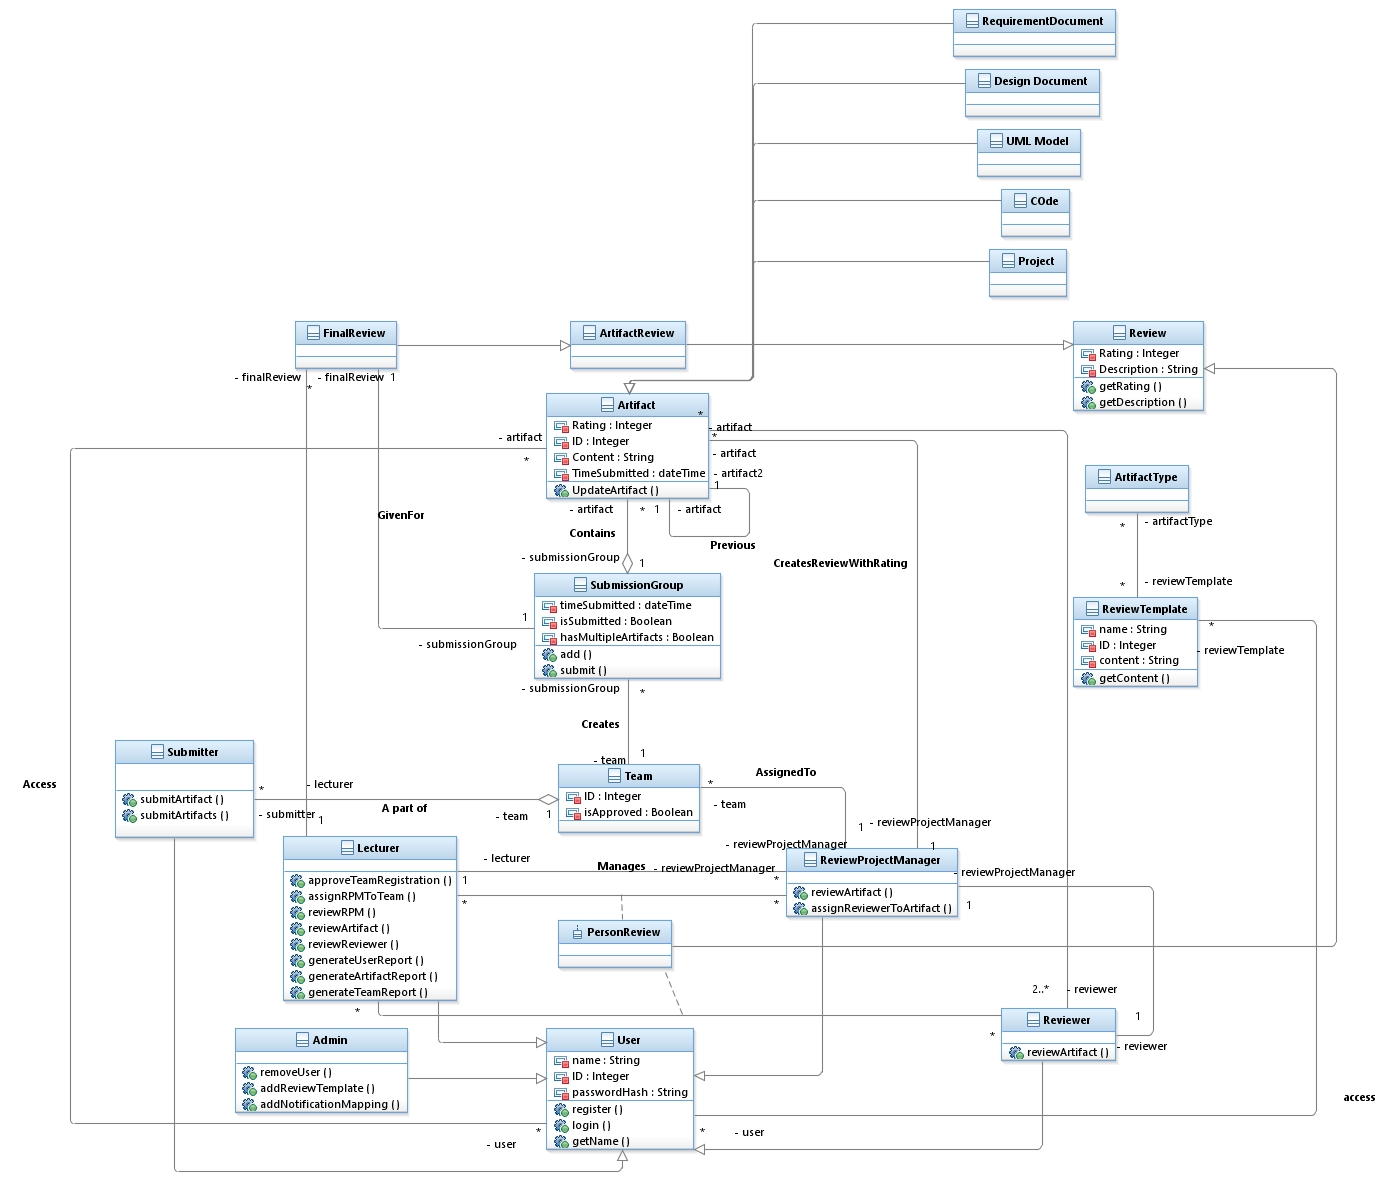
\includegraphics[width=16cm]{content/CD.jpeg}
\centering

\caption{Class Diagram for SoftProj System}
\end{figure}
  \newpage
 \section{Sequence Diagrams and Corresponding Operation Contract }   
\subsection*{SD 1: Review Artifact (Reviewer)}

\begin{figure}[h]
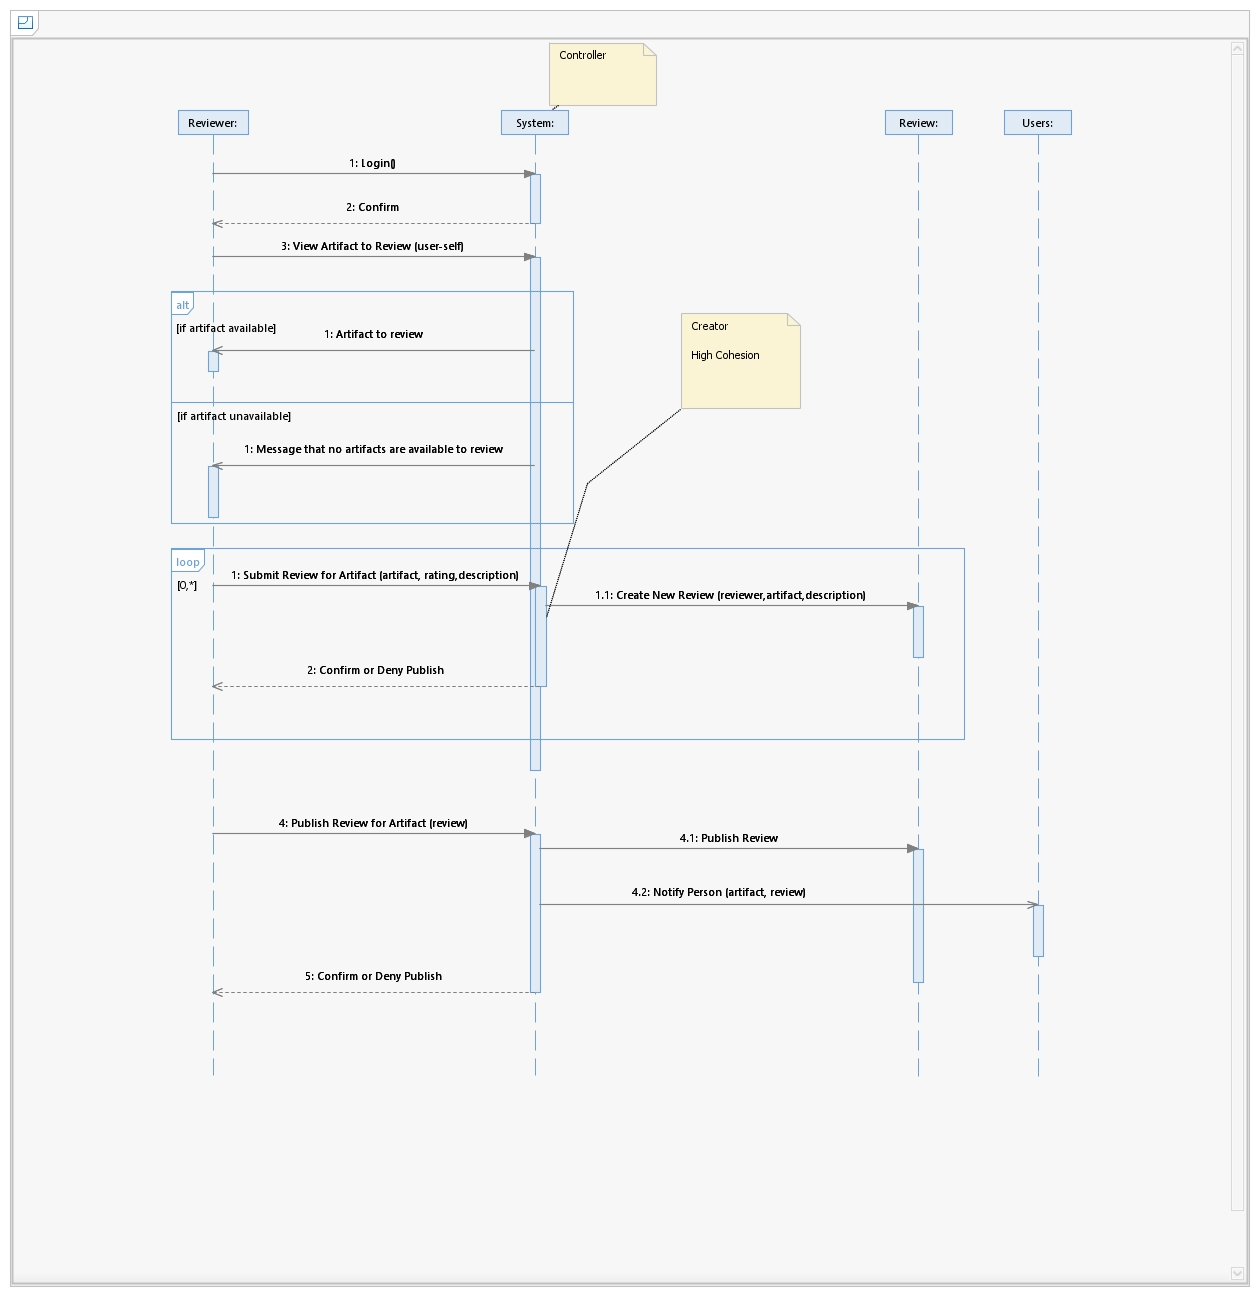
\includegraphics[width=13cm]{SD_ReviewArtifact_5.jpeg}
\centering
\caption{Sequence Diagram for \textbf{Review Artifact (Reviewer)} with GRASP indicator}
\end{figure}


%OC1


\subsection*{Operation Contracts:}
\subsection*{View Artifact To Review (user-self)}
\subsubsection*{Preconditions:}
\begin{itemize}
\itemsep-1em 
    \item Reviewer \textbf{r} was identified and authenticated. 
    \item Reviewer \textbf{r} had been assigned by an RPM \textbf{rpm} to review an Artifact \textbf{a} submitted by a Team \textbf{t}.
    \item Reviewer \textbf{r} was notified by the System that they had been assigned to review an Artifact \textbf{a}.
\end{itemize}



\subsubsection*{Postconditions:}
\begin{itemize}
\itemsep-1em 
    \item Reviewer \textbf{r} was able to see the Artifact \textbf{a}.
\end{itemize}



\subsection*{Submit Review for Artifact (artifact, rating, description) }
\subsubsection*{Preconditions:}
\begin{itemize}
\itemsep-1em 
    \item Reviewer \textbf{r} was identified and authenticated. 
    \item Reviewer \textbf{r} had been assigned by an RPM \textbf{rpm} to review an Artifact \textbf{a} submitted by a Team \textbf{t}.
    \item Reviewer \textbf{r} was notified by the System \textbf{s} that he/she had been assigned to review an Artifact \textbf{a}.
    \item Reviewer \textbf{r} provided new content for either rating or description.
\end{itemize}



\subsubsection*{Postconditions:}
\begin{itemize}
\itemsep-1em 
    \item New Review \textbf{nr} had been created with provided rating and description
    \item Review \textbf{nr} had been associated with the Artifact \textbf{a} and the Reviewer \textbf{r}.
\end{itemize}




\subsection*{Publish Review for Artifact (review)}
\subsubsection*{Preconditions:}
\begin{itemize}
\itemsep-1em 
    \item Reviewer \textbf{r} was identified and authenticated.
    \item Review \textbf{nr} was referred to a completed Review with both description and rating.
\end{itemize}



\subsubsection*{Postconditions:}
\begin{itemize}
\itemsep-1em 
    \item Review \textbf{nr} had been set to be published
    \item Review was \textbf{nr} visible to all associated Users.
    \item Associated Users had been notified if they were subscribed to notifications.
\end{itemize}






\newpage




\subsection*{SD 2: Assign Team to RPM}



\begin{figure}[h]
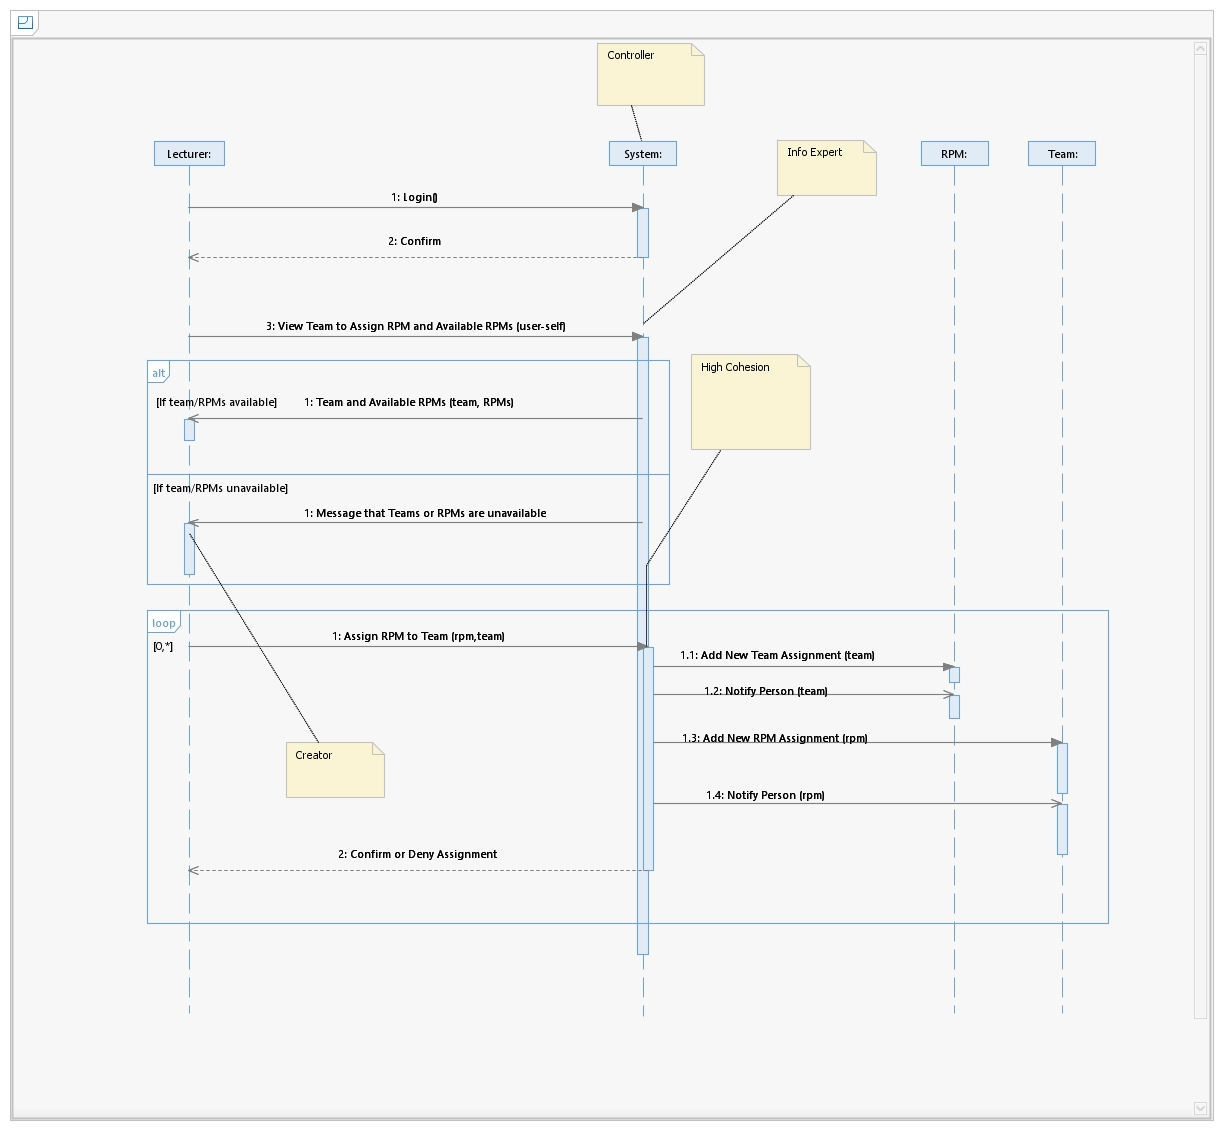
\includegraphics[width=14cm]{SD_AssignTeamToRPM.jpeg}
\centering
\caption{Sequence Diagram for \textbf{Assign Team to RPM} with GRASP indicator}
\end{figure}

%OC2



\subsection*{Operation Contracts:}
\subsection*{View Team to Assign RPM and Available RPMs (user-self)}
\subsubsection*{Preconditions:}
\begin{itemize}
\itemsep-1.5em 
    \item Lecturer \textbf{l} was identified and authenticated. 
    \item Fist Artifact \textbf{a} had been submitted by Team \textbf{t}.
    \item Lecturer noticed that the Team \textbf{t} submitted their first Artifact \textbf{a}.
\end{itemize}



\subsubsection*{Postconditions:}
\begin{itemize}
\itemsep-1.5em 
    \item Submitted first Artifact \textbf{a} of Team \textbf{t} was seen by Lecturer \textbf{l}.
    \item Available RPMs was seen by Lecturer \textbf{l}.
\end{itemize}



\subsection*{Assign RPM to Team (rpm, team)}
\subsubsection*{Preconditions:}
\begin{itemize}
\itemsep-1.5em 
    \item Lecturer \textbf{l} was identified and authenticated.
    \item Artifact \textbf{a} had been submitted by team \textbf{t} .
    \item Team \textbf{t} had not already been assigned to an RPM \textbf{rpm}.
    \item RPM \textbf{rpm} was available.
    \item An RPM \textbf{rpm} had been chosen by Lecturer \textbf{l} to be assigned to the team \textbf{t}.
\end{itemize}



\subsubsection*{Postconditions:}
\begin{itemize}
\itemsep-1.5em 
    \item The RPM \textbf{rpm} and Team \textbf{t} was associated with one another.
    \item The RPM \textbf{rpm} and Team \textbf{t} had been notified of their new association.
\end{itemize}




\subsection*{Add New Team Assignment (team)}
\subsubsection*{Context:} RPM
\subsubsection*{Preconditions:}
\begin{itemize}
\itemsep-1.5em 
    \item RPM \textbf{rpm} was available
    \item Team \textbf{t} had not been assigned an RPM.
\end{itemize}



\subsubsection*{Postconditions:}
\begin{itemize}
\itemsep-1.5em 
    \item The RPM \textbf{rpm} had been assigned to the Team \textbf{t}.
    \item The RPM  \textbf{rpm} received notifications for Team \textbf{t}’s submitted Artifacts.
\end{itemize}



\subsection*{Add New RPM Assignment (rpm)}
\subsubsection*{Context:} Team
\subsubsection*{Preconditions:}
\begin{itemize}
\itemsep-1.5em 
    \item Team \textbf{t} had not yet been assigned an RPM \textbf{rpm}.
    \item RPM \textbf{rpm} was available
\end{itemize}



\subsubsection*{Postconditions:}
\begin{itemize}
\itemsep-1.5em 
    \item Team \textbf{t} had been assigned to the RPM \textbf{rpm}.
    \item Team \textbf{t} received notifications for RPM \textbf{rpm}’s Reviews of their Artifacts.
\end{itemize}







\subsection*{SD 3: Register Team}

\begin{figure}[h]
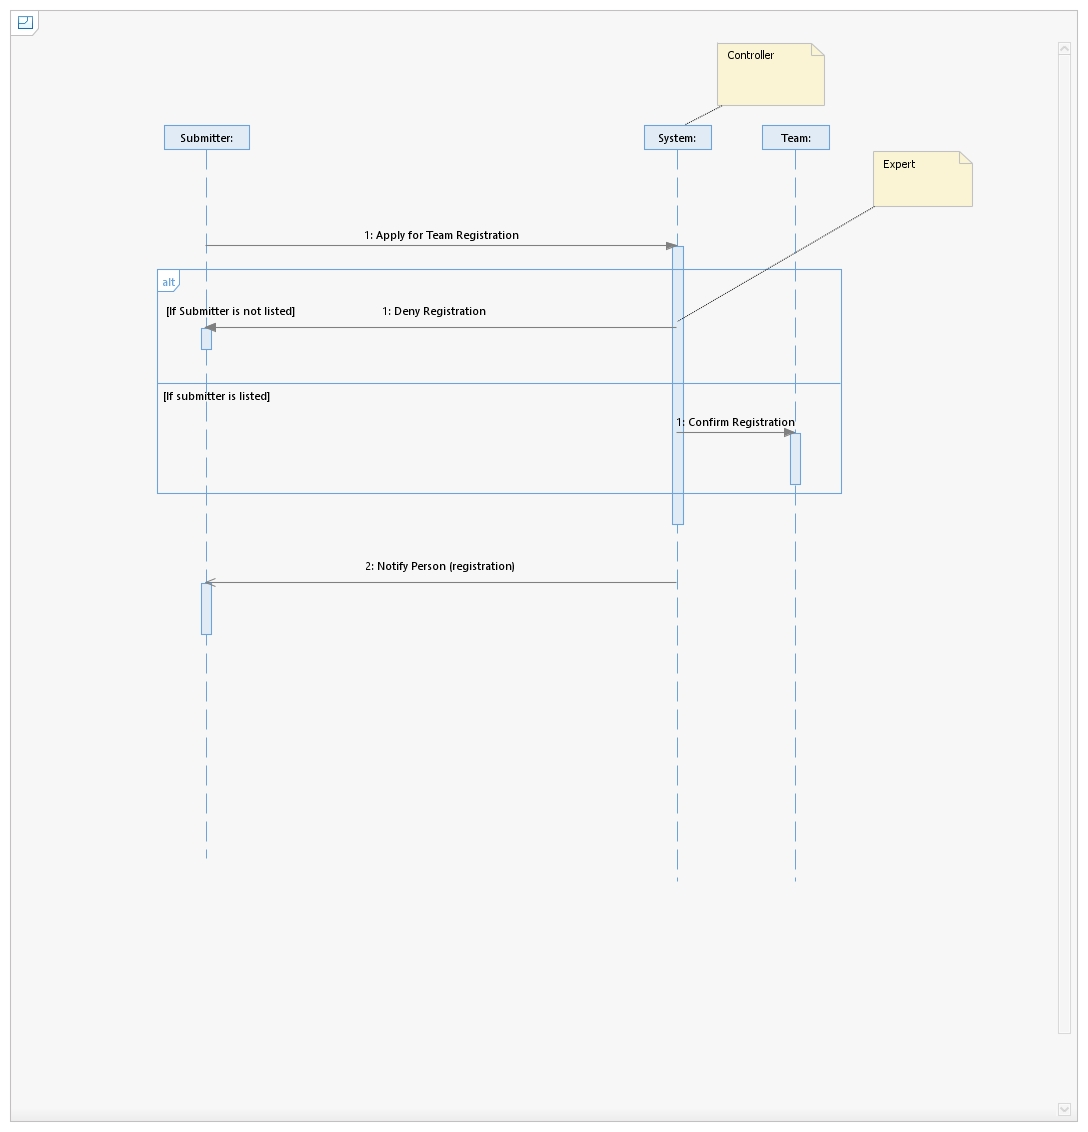
\includegraphics[width=13cm]{SD_RegisterTeam.jpeg}
\centering
\caption{Sequence Diagram for \textbf{Register Team} with GRASP indicator}
\end{figure}



%OC3
\subsection*{Operation Contracts:}
\subsection*{Apply for Team Registration}

\subsubsection*{Preconditions:}
\begin{itemize}
\itemsep-1.5em 
    \item Submitter \textbf{sub} was listed in the database.
   
\end{itemize}



\subsubsection*{Postconditions:}
\begin{itemize}
\itemsep-1.5em 
    \item Registration \textbf{r} had been confirmed.
    \item Team \textbf{t} had been listed to database.
    \item Submitter \textbf{sub} had been notified.
\end{itemize}

\newpage








\subsection*{SD 4: Submit Artifact for Review}

\begin{figure}[h]
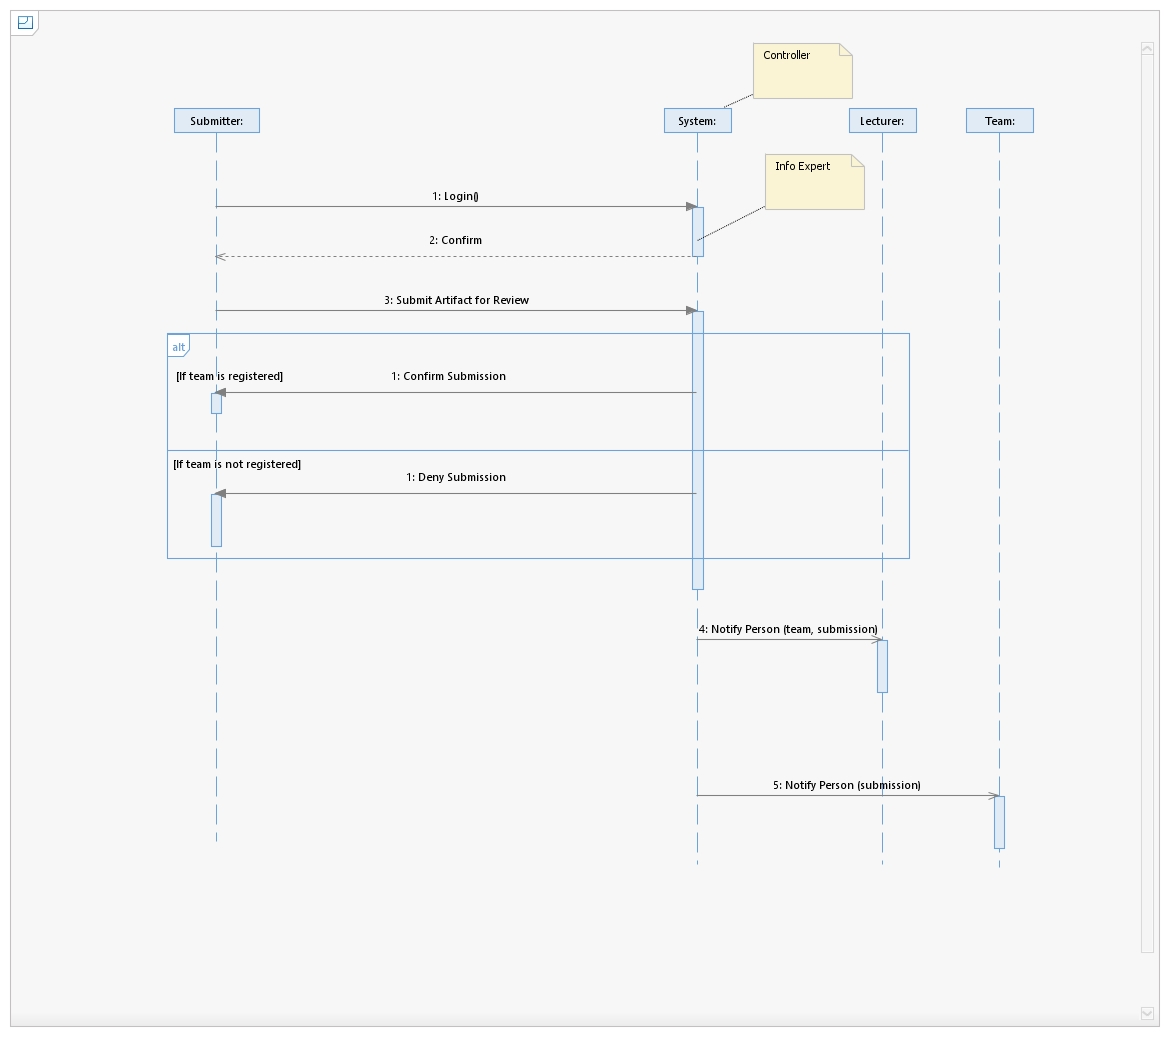
\includegraphics[width=14cm]{SD_SubmitArtifactForReview.jpeg}
\centering
\caption{Sequence Diagram for \textbf{Submit Artifact for Review} with GRASP indicator}
\end{figure}






%OC4
\subsection*{Operation Contracts:}
\subsection*{Login()}

\subsubsection*{Preconditions:}
\begin{itemize}
\itemsep-1.5em 
    \item Instance of Submitter \textbf{sub} was created.
   
\end{itemize}



\subsubsection*{Postconditions:}
\begin{itemize}
\itemsep-1.5em 
    \item Submitter \textbf{sub} was identified and authenticated.

\end{itemize}



\subsection*{Submit Artifact for Review}

\subsubsection*{Preconditions:}
\begin{itemize}
\itemsep-1.5em 
    \item Submitter \textbf{sub} was authenticated.
    \item Team \textbf{t} was registered
  
   
\end{itemize}



\subsubsection*{Postconditions:}
\begin{itemize}
\itemsep-1.5em 
   \item An artifact \textbf{a} was submitted.
   \item Team \textbf{t} was notified.
   \item Lecturer \textbf{l} was notified.

\end{itemize}




\subsection*{SD 5: Assign Reviewers to Artifact(s)}

\begin{figure}[h]
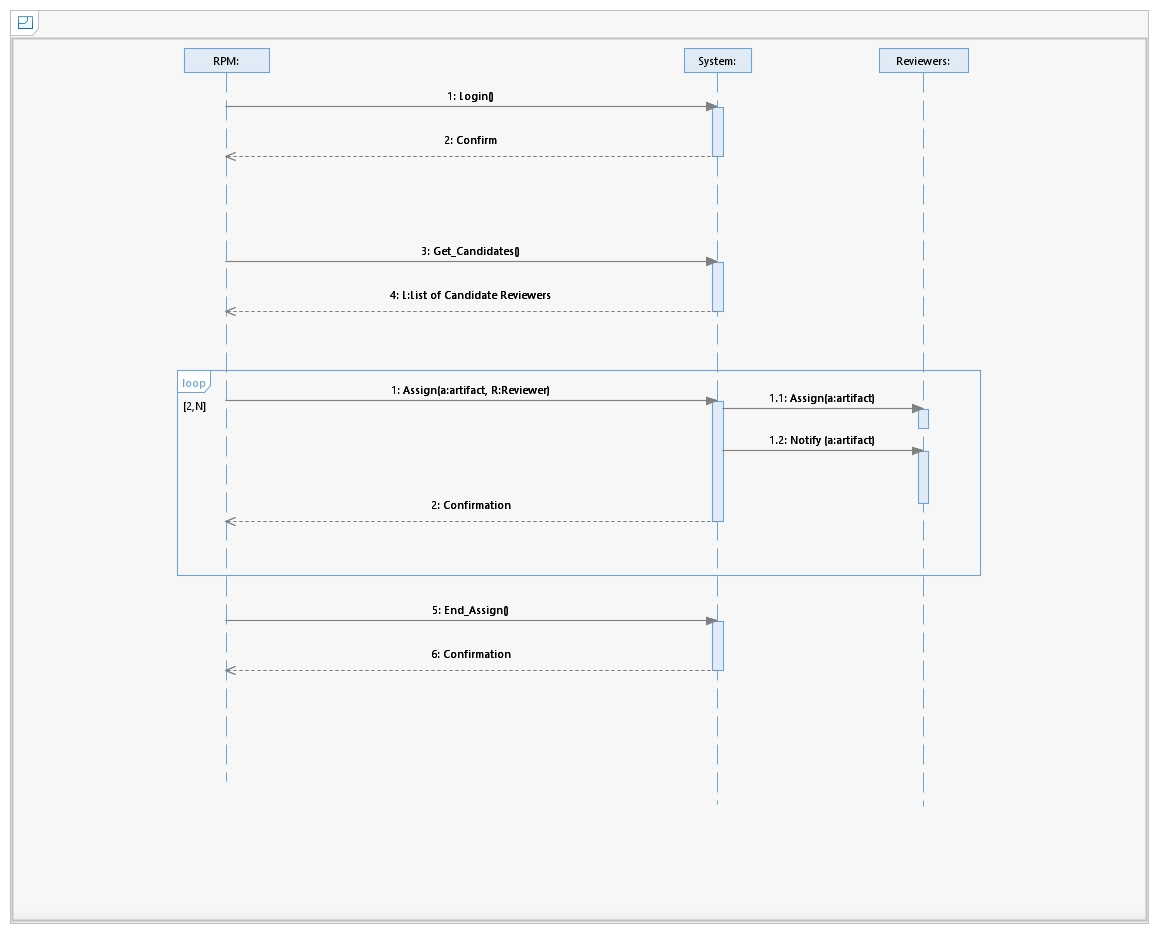
\includegraphics[width=16cm]{SD_AssignReviewerstoArtifacts.jpeg}
\centering
\caption{Sequence Diagram for \textbf{Assign Reviewers to Artifact(s)}}
\end{figure}


%UC5

\subsection*{Operation Contracts:}
\subsection*{login()}

\subsubsection*{Preconditions:}
\begin{itemize}
\itemsep-1.5em 
    \item Instance of RPM \textbf{rpm} was created.
    
  
   
\end{itemize}



\subsubsection*{Postconditions:}
\begin{itemize}
\itemsep-1.5em 
   \item RPM \textbf{rpm} was identified and authenticated.

\end{itemize}





\subsection*{get\_candidates()}

\subsubsection*{Preconditions:}
\begin{itemize}
\itemsep-1.5em 
    \item RPM \textbf{rpm} was authenticated.
    
  
   
\end{itemize}



\subsubsection*{Postconditions:}
\begin{itemize}
\itemsep-1.5em 
   \item List of candidate reviewers were shown.

\end{itemize}








\subsection*{assign(a:artifact, r: Reviewer )}

\subsubsection*{Preconditions:}
\begin{itemize}
\itemsep-1.5em 
    \item RPM \textbf{rpm} was authenticated.
    \item An instance of Artifact \textbf{a} was created and initialized.
    \item Reviewer \textbf{r} was authenticated.
  
   
\end{itemize}



\subsubsection*{Postconditions:}
\begin{itemize}
\itemsep-1.5em 
   \item Instance \textbf{a} was associated with \textbf{r}.

\end{itemize}





\subsection*{end\_assign()}

\subsubsection*{Preconditions:}
\begin{itemize}
\itemsep-1.5em 
    \item RPM \textbf{ rpm} was authenticated.
    
  
   
\end{itemize}



\subsubsection*{Postconditions:}
\begin{itemize}
\itemsep-1.5em 
   \item Confirmation was sent to RPM \textbf{rpm}. 

\end{itemize}









\newpage



\subsection*{SD 6: Rate Artifact (RPM)}

\begin{figure}[h]
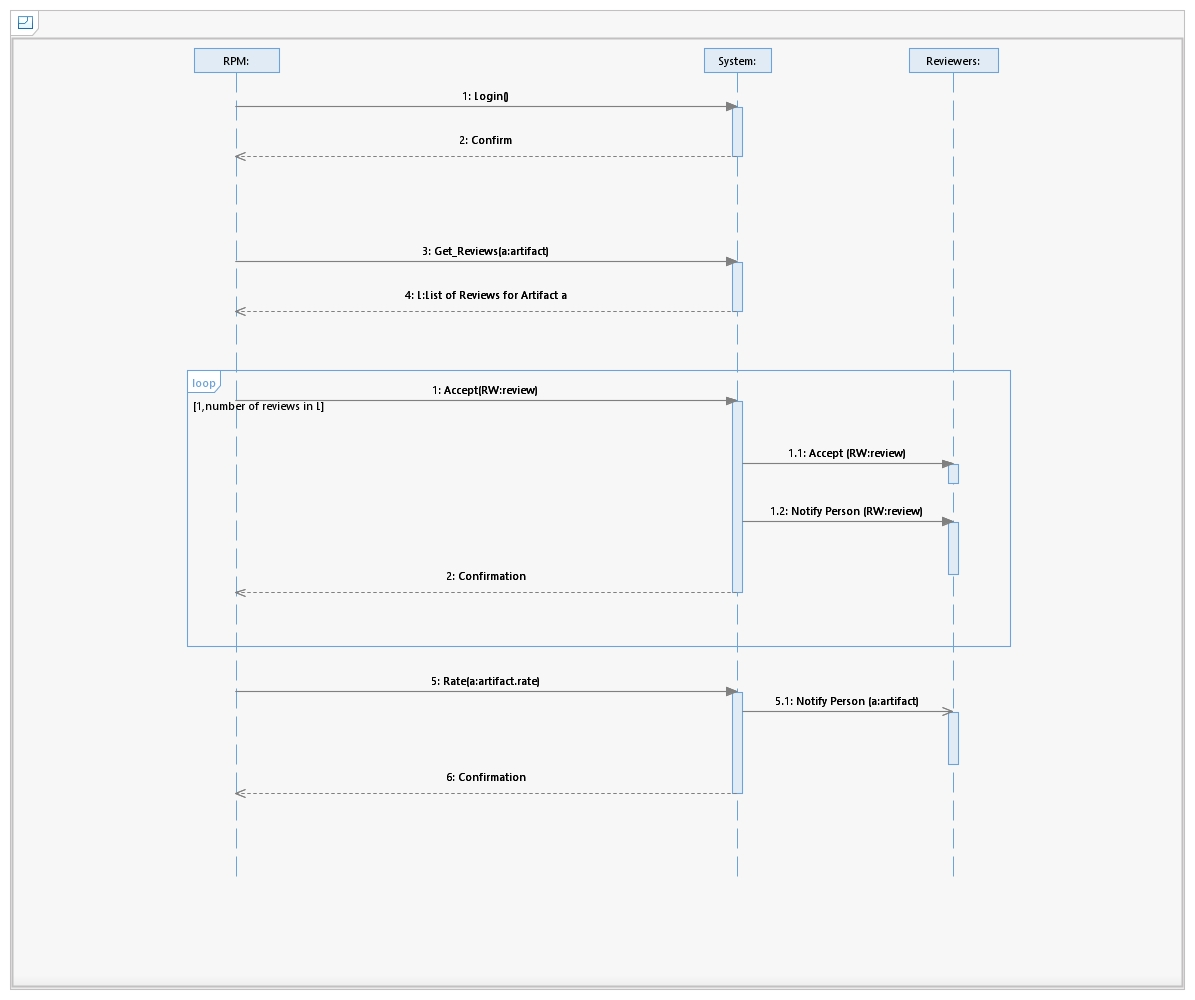
\includegraphics[width=16cm]{SD_RateArtifact.jpeg}
\centering
\caption{Sequence Diagram for \textbf{Rate Artifact (RPM)}}
\end{figure}





%OC6



\subsection*{Operation Contracts:}
\subsection*{login()}

\subsubsection*{Preconditions:}
\begin{itemize}
\itemsep-1.5em 
    \item Instance of RPM \textbf{rpm} was created.
    
  
   
\end{itemize}



\subsubsection*{Postconditions:}
\begin{itemize}
\itemsep-1.5em 
   \item RPM \textbf{rpm} was identified and authenticated.

\end{itemize}





\subsection*{get\_reviews(a:artifact)}

\subsubsection*{Preconditions:}
\begin{itemize}
\itemsep-1.5em 
    \item RPM \textbf{rpm} was authenticated.
    \item An instance of Artifact \textbf{a} was created, initialized and associated with multiple (2...N) instances of Reviewer.
    \item Multiple (2...N) instances of Review were created, initialized and each was associated with one instance of Reviewer and one instance of Artifact.
    
  
   
\end{itemize}



\subsubsection*{Postconditions:}
\begin{itemize}
\itemsep-1.5em 
   \item List of reviews for Artifact \textbf{a} were shown.

\end{itemize}








\subsection*{accept(RW: Review)}

\subsubsection*{Preconditions:}
\begin{itemize}
\itemsep-1.5em 
    \item RPM \textbf{rpm} was authenticated.
    \item An instance of Review \textbf{RW} was created, initialized and associated with an instance of Artifact \textbf{a}
    \item An instance of Review \textbf{RW} was associated with an instance of Reviewer \textbf{r}.
  
   
\end{itemize}



\subsubsection*{Postconditions:}
\begin{itemize}
\itemsep-1.5em 
   \item \textbf{RW.isAccepted} was set to true.

\end{itemize}





\subsection*{rate(a:artifact, rate)}

\subsubsection*{Preconditions:}
\begin{itemize}
\itemsep-1.5em 
    \item RPM \textbf{rpm} was authenticated.
    \item An instance of Artifact \textbf{a} was created and initialized.
    \item \textbf{RW.isAccepted} for all Review \textbf{RW} associated with Artifact \textbf{a} was set to true.
    
  
   
\end{itemize}



\subsubsection*{Postconditions:}
\begin{itemize}
\itemsep-1.5em 
   \item \textbf{a.rate} was set to rate. 

\end{itemize}






\newpage

\subsection*{SD 7: Rate Artifact 2 (Lecturer)}

\begin{figure}[h]
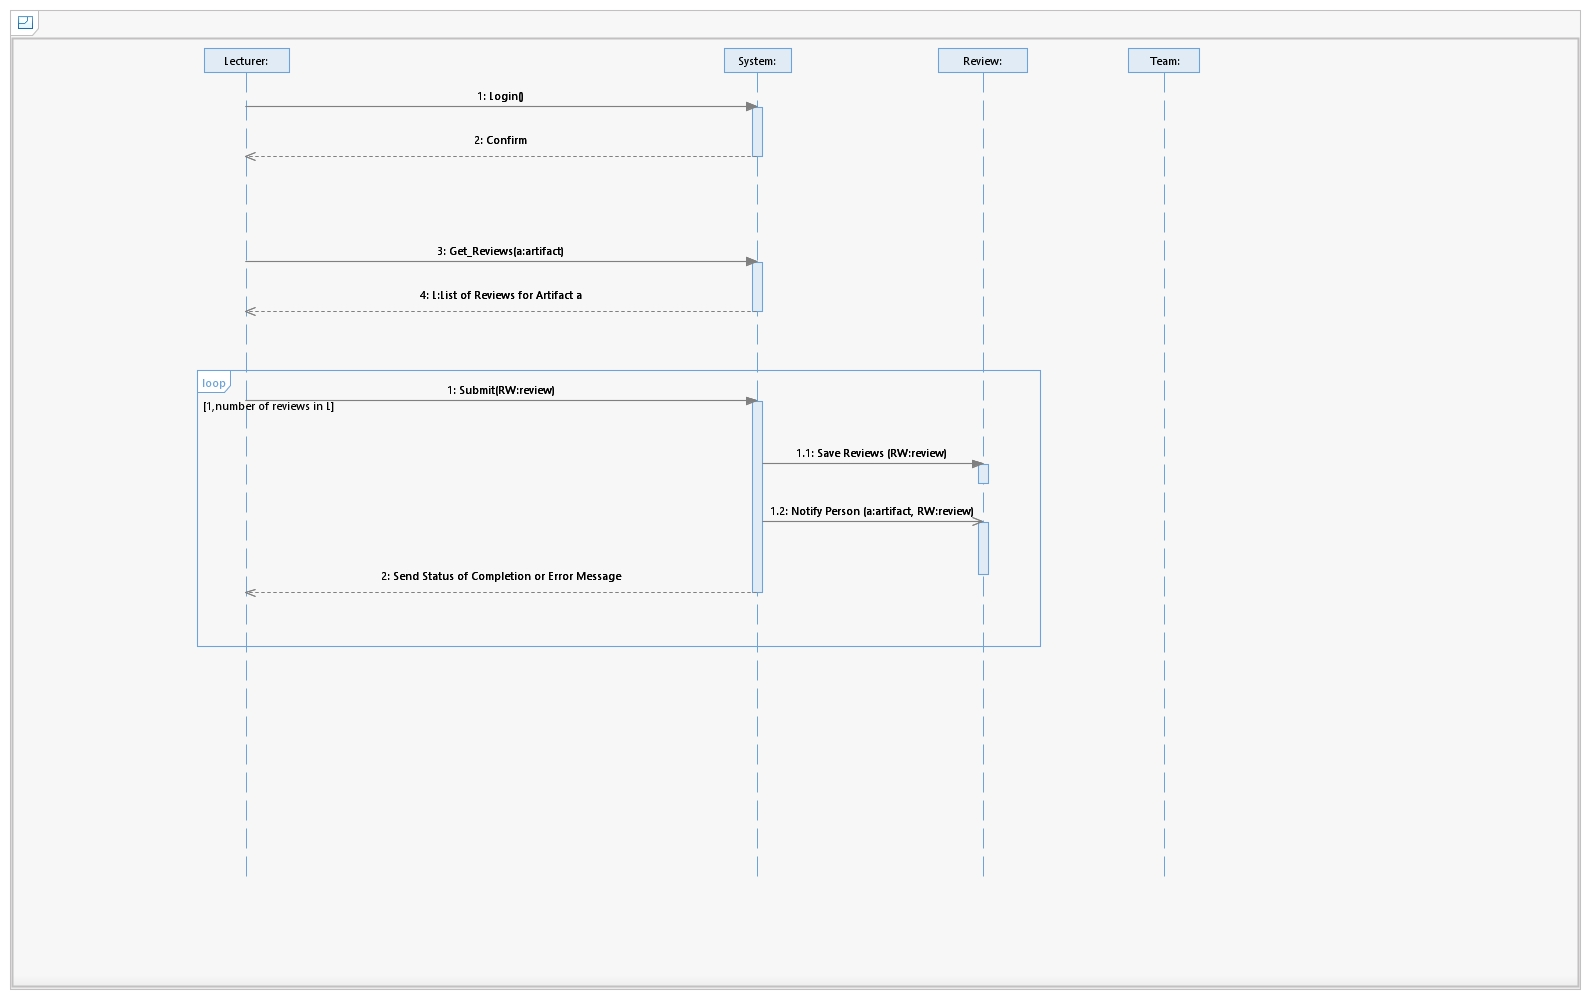
\includegraphics[width=16cm]{SD_RateArtifact(Lecturer).jpeg}
\centering
\caption{Sequence Diagram for \textbf{Rate Artifact 2 (Lecturer)}}
\end{figure}

\subsection*{Operation Contracts:}
\subsection*{View Reviews to Rate Artifact(user)}
\subsubsection*{Preconditions:}
\begin{itemize}
\itemsep-1.5em 
    \item Lecturer \textbf{l} was identified and authenticated.
    \item Lecturer \textbf{l} was notified by the System that he has been assigned to review an Artifact \textbf{a}.
\end{itemize}



\subsubsection*{Postconditions:}
\begin{itemize}
\itemsep-1.5em 
    \item Lecturer \textbf{l} can see the Artifact \textbf{a} they need to review.
    \item Lecturer \textbf{l} can see the reviews given by the RPM \textbf{rpm} and the Reviewers for that Artifact \textbf{a}.
\end{itemize}

\newpage

\subsection*{Submit Reviews (Reviews)}
\subsubsection*{Preconditions:}
\begin{itemize}
\itemsep-1.5em 
    \item Lecturer \textbf{l} was identified and authenticated.
    \item Lecturer \textbf{l } was notified by the System that he had been assigned to review an Artifact \textbf{a}.
    \item Lecturer \textbf{l} was able to view the reviews given by the RPM \textbf{rpm} \& the Reviewers.
    \item Lecturer \textbf{l} had provided reviews for Artifact \textbf{a}, RPM and each of the Reviewers
\end{itemize}



\subsubsection*{Postconditions:}
\begin{itemize}
\itemsep-1.5em 
    \item The system \textbf{s} had created a new review for each of the associated user and object
    \item Review \textbf{RW} had been associated with Artifact \textbf{a}, RPM \textbf{rpm}, Reviewers \textbf{r}
\end{itemize}





\section{Architectural Model}

\begin{figure}[h]
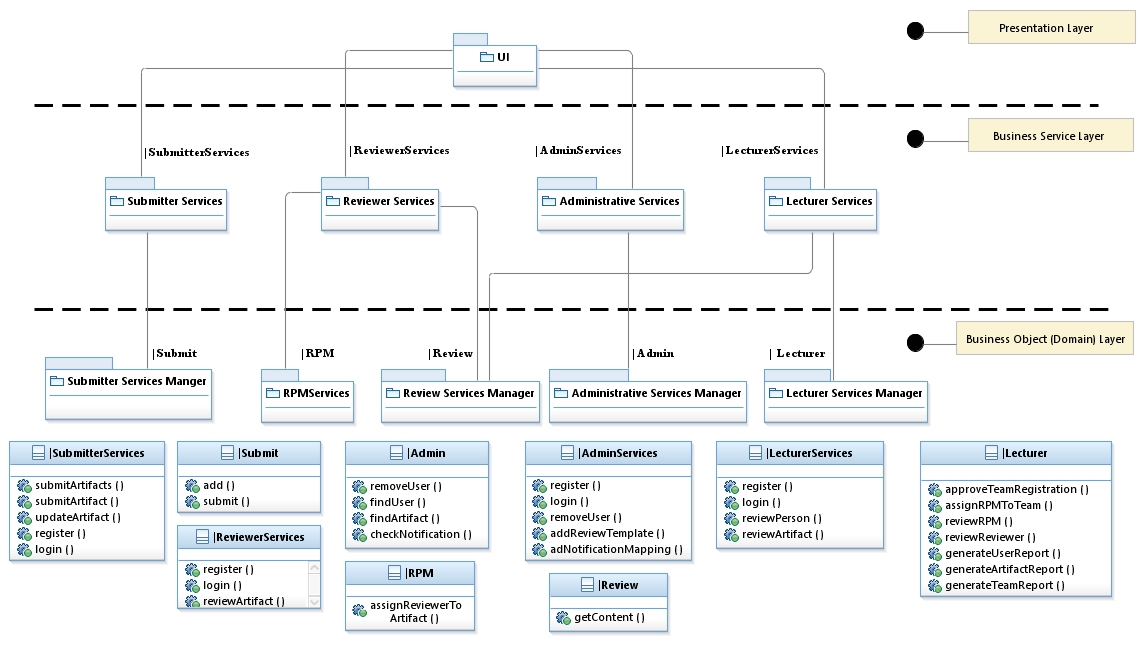
\includegraphics[width=15cm]{Architectural.jpeg}
\centering
\caption{Architectural Model of SoftProj System}
\centering
\end{figure}
\vfill
\hspace{0pt}
\pagebreak




\newpage

\section{Package Diagram}

\begin{figure}[h]
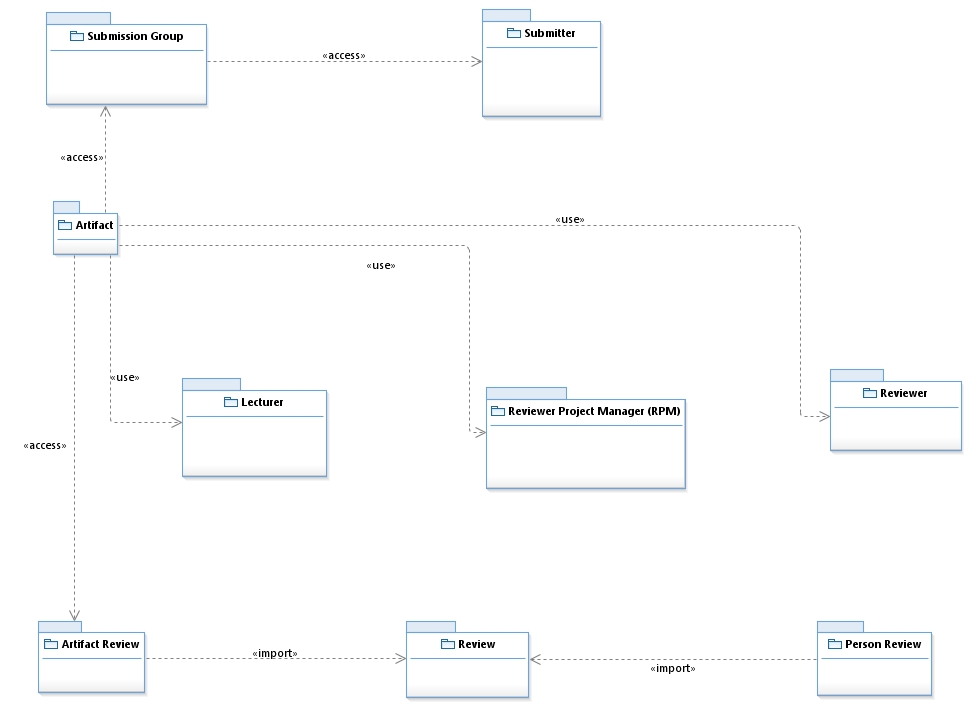
\includegraphics[width=15cm]{PackageDiagram.jpeg}
\centering
\caption{Package Diagram for SoftProj System}
\centering
\end{figure}



